%% -*- coding: utf-8 -*-
\documentclass[12pt,a4paper]{scrartcl} 
\usepackage[utf8]{inputenc}
\usepackage[english,russian]{babel}
\usepackage{indentfirst}
\usepackage{misccorr}
\usepackage{graphicx}
\usepackage{amsmath}
\usepackage{float}

\usepackage{xcolor}
\usepackage{hyperref}
\hypersetup{colorlinks,
  pdftitle={The title of your document},
  pdfauthor={Your name},
  allcolors=[RGB]{010 090 200}}

\begin{document}
\begin{titlepage}
  \begin{center}

    Санкт-Петербургский политехнический университет Петра Великого

    \vspace{0.25cm}
    
    Институт прикладной математики и механики
    
    Кафедра «Прикладная математика»
    \vfill

	\vspace{0.25cm}
	    Отчёт\\
	по лабораторной работе №1\\
	по дисциплине\\
	«Математическая статистика»

  \bigskip

\end{center}
\vfill

\newlength{\ML}
\settowidth{\ML}{«\underline{\hspace{0.7cm}}» \underline{\hspace{2cm}}}
\hfill\begin{minipage}{0.4\textwidth}
  Выполнил студент\\ В.\,А.~Рыженко\\
\end{minipage}%
\bigskip

\hfill\begin{minipage}{0.4\textwidth}
  Проверил:\\
к.ф.-м.н., доцент\\
Баженов Александр Николаевич\\
\end{minipage}%
\vfill

\begin{center}
  Санкт-Петербург, 2020 г.
\end{center}
\end{titlepage}

\tableofcontents
\listoffigures
\newpage

\section{Постановка задачи}
 
Для 5 распределений:
\begin{itemize}
 \item Нормальное распределение N(x, 0, 1)
 \item Распределение Коши C(x, 0, 1)
 \item Распределение Лапласа L(x, 0, $\frac{1}{\sqrt2}$)
 \item Постановка задач исследованияРаспределение Пуассона P(k, 10)
 \item Равномерное распределение U(x, $-\sqrt{3}, \sqrt{3}$) 
\end{itemize}
 
Сгенерировать выборки размером 10, 50 и 1000 элементов.
Построить на одном рисунке гистограмму и график плотности распределения.

\section{Распределения}

\begin{itemize}
\begin{item}
Нормальное распределение
\begin{equation}\label{eq:Normal}
\centering
 N(x, 0, 1) = \frac{1}{\sqrt{2\pi} } e^{-\frac{x^2}2}
\end{equation}
\end{item}

\begin{item}
Распределение Коши
\begin{equation}\label{eq:Cauchy}
\centering
 C(x, 0, 1) = \frac{1}{\pi} \frac{1}{x^2 + 1}
\end{equation}
\end{item}

\begin{item}
Распределение Лапласа
\begin{equation}\label{eq:Laplace}
\centering
L(x, 0, \frac{1}{\sqrt2}) = \frac{1}{\sqrt{2} } e^{\sqrt2|x|}
\end{equation}
\end{item}

\begin{item}
Распределение Пуассона
\begin{equation}\label{eq:Poisson}
\centering
P(k, 10) = \frac{10^k}{k! } e^{-10}
\end{equation}
\end{item}

\begin{item}
Равномерное распределение
\begin{equation}\label{eq:Uniform}
\centering
U(x, -\sqrt{3}, \sqrt{3})  = 
\begin{cases}
\frac{1}{2\sqrt3}, &\mbox{при } |x| \leq \sqrt3 \\ 0 , &\mbox{при } |x| \textgreater \sqrt3
\end{cases}
\end{equation}
\end{item}
\end{itemize}

\section {Реализация}
Лабораторная работа выполнена с помощью встроенных средств языка программирования Python в среде разработки Jupyter Notebook. Исходный код лабораторной
работы приведён в приложении.
 
\section{Результаты}
\begin{figure}[H]
  \centering
  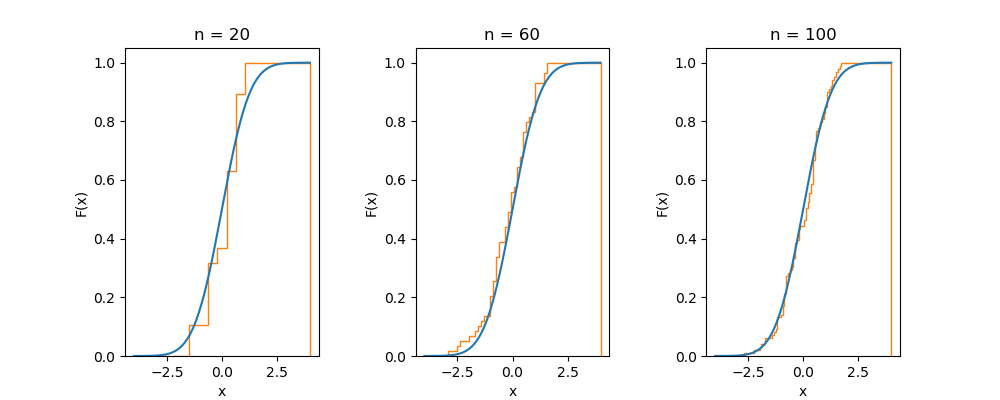
\includegraphics[width=0.8\textwidth]{Normal.png}
  \caption{Нормальное распределение ~\eqref{eq:Normal}}
 
\end{figure}
\begin{figure}[H]
  \centering
  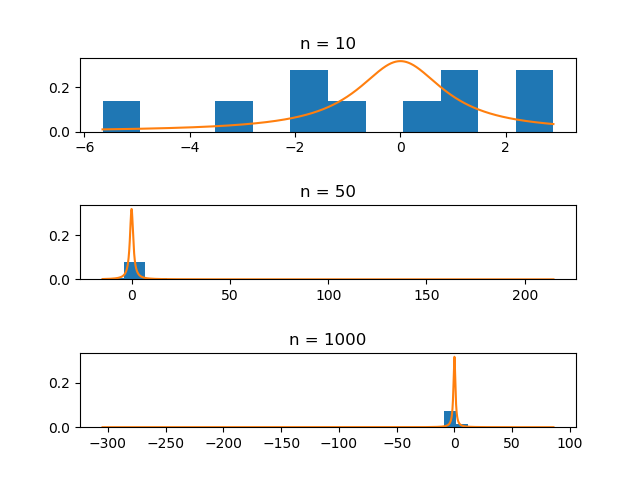
\includegraphics[width=0.8\textwidth]{Cauchy.png}
  \caption{Распределение Коши ~\eqref{eq:Cauchy}}
\end{figure}
\begin{figure}[H]
\centering
  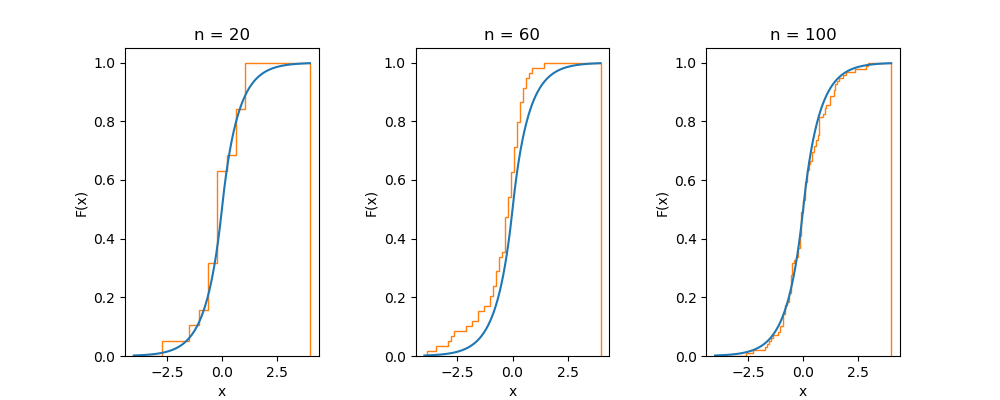
\includegraphics[width=0.8\textwidth]{Laplace.png}
  \caption{Распределение Лапласа ~\eqref{eq:Laplace}}
\end{figure}
\begin{figure}[H]
  \centering
  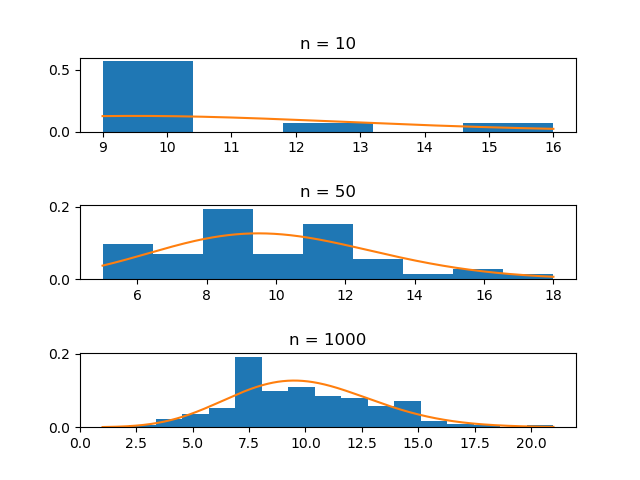
\includegraphics[width=0.8\textwidth]{Poisson.png}
  \caption{Распределение Пуассона ~\eqref{eq:Poisson}}
\end{figure}
\begin{figure}[H]
  \centering
  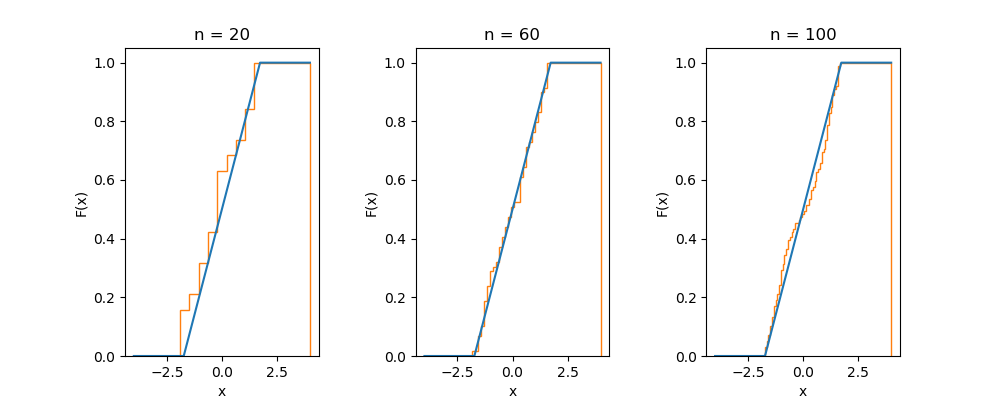
\includegraphics[width=0.8\textwidth]{Uniform.png}
  \caption{Равномерное распределение ~\eqref{eq:Uniform}}
\end{figure}

\section{Обсуждение}
Из графиков видна чёткая зависимость, увеличение выборки увеличивает точность аппроксимации исходного распределения для всех распределений кроме Коши~\eqref{eq:Cauchy}.

\section{Приложения}
Репозиторий на GitHub с релизацией: \href{https://github.com/WiillyWonka/MatStat}{github.com}.
\end{document}
